\documentclass[pdflatex,compress]{beamer}

%\usetheme[dark,framenumber,totalframenumber]{ElektroITK}
\usetheme[darktitle,framenumber,totalframenumber]{ElektroITK}
\usepackage{graphicx}
\usepackage{multicol}

\title{Data Communications}
\subtitle{Chapter 4 - Transmission Media}

\author{Mifta Nur Farid}

\begin{document}

\maketitle

\begin{frame}
	\frametitle{Design Factors Determining Data Rate and Distance}
	\begin{itemize}
		\item \textbf{Bandwidth}\\
		Higher bandwidth gives higher data rate
		\item \textbf{Transmission impairments}\\
		Impairments, such as attenuation, limit the distance
		\item \textbf{Interference}\\
		Overlapping frequency bands can distort or wipe out a signal
		\item \textbf{Number of receivers}\\
		More receivers introduces more attenuation
	\end{itemize}
\end{frame}

\begin{frame}
	\begin{center}
		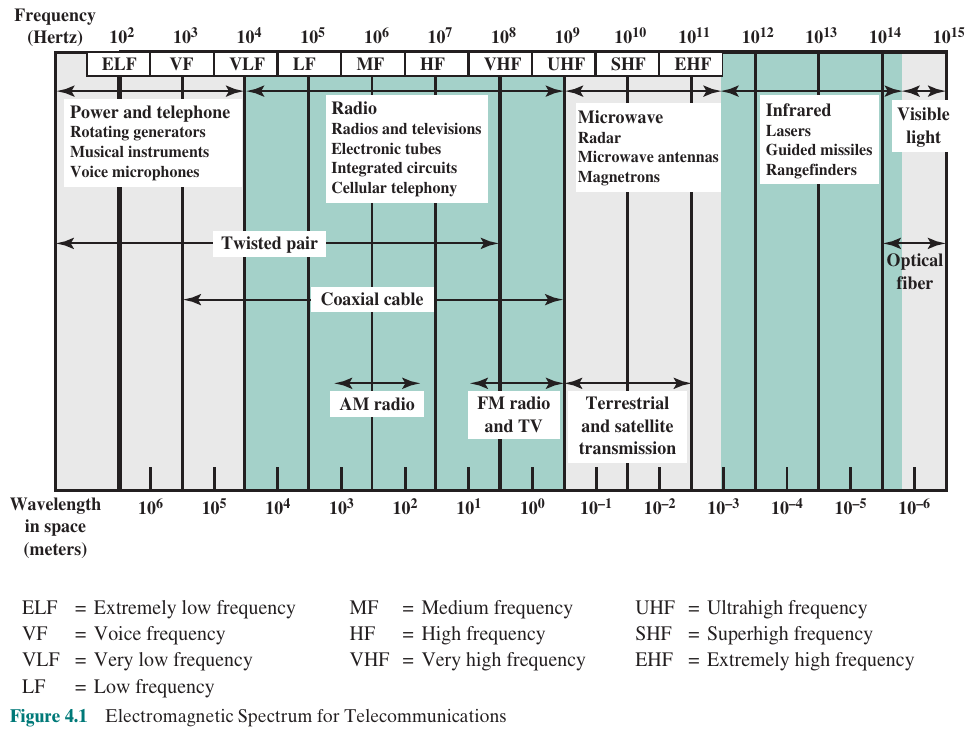
\includegraphics[width=0.9\linewidth]{img/img01}
	\end{center}
\end{frame}

\begin{frame}
	\begin{center}
		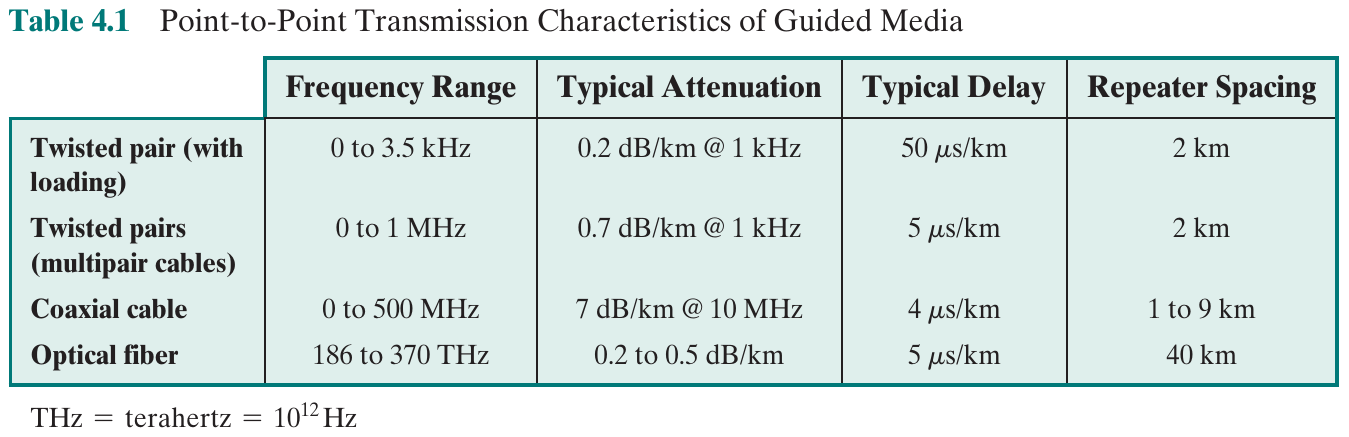
\includegraphics[width=\linewidth]{img/img02}
	\end{center}
\end{frame}

\begin{frame}
	\begin{center}
		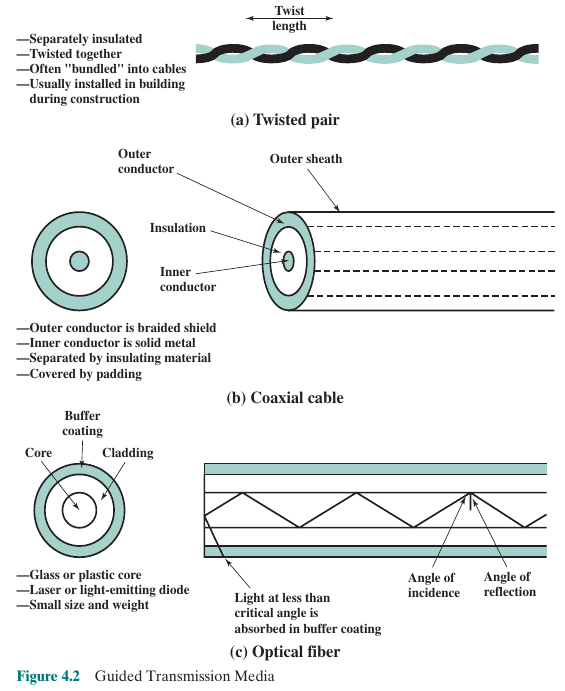
\includegraphics[width=0.5\linewidth]{img/img03a}
	\end{center}
\end{frame}

\begin{frame}
	\frametitle{Twisted Pair}
	\begin{center}
		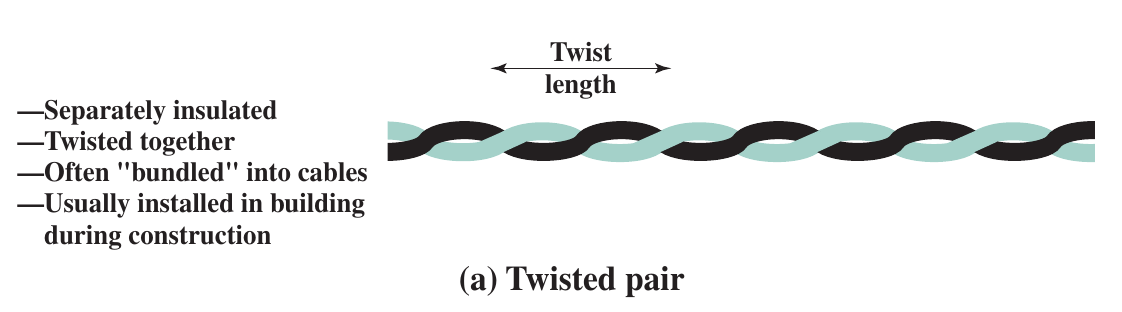
\includegraphics[width=0.8\linewidth]{img/img03}
	\end{center}
	Twisted pair is the least expensive and most widely used guided transmission medium
	\begin{itemize}
		\item Consists of two insulated copper wires arranged in a regular spiral pattern
		\item A wire pair acts as a single communication link
		\item Pairs are bundled together into a cable
		\item Most commonly used in the telephone network and for communications within buildings
	\end{itemize}
\end{frame}

\begin{frame}
	\begin{center}
		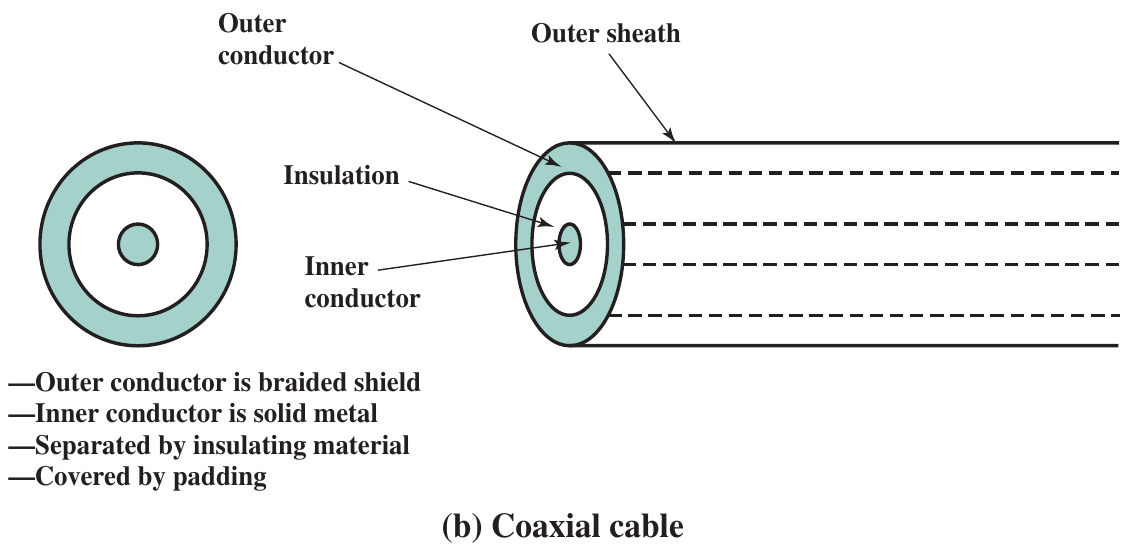
\includegraphics[width=\linewidth]{img/img04}
	\end{center}
\end{frame}

\begin{frame}
	\begin{center}
		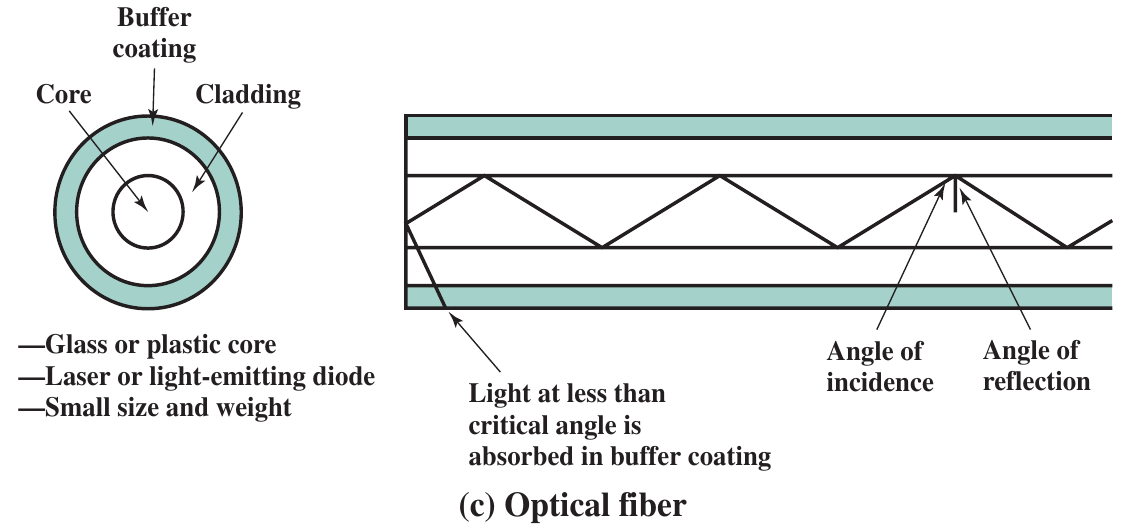
\includegraphics[width=\linewidth]{img/img05}
	\end{center}
\end{frame}

\begin{frame}
	\frametitle{Summary}

\end{frame}

\begin{frame}
	\frametitle{Tugas Mandiri}
	\begin{itemize}
		\item Stallings, W. (2014). Data and Computer Communications, 10th Edition, New Jersey: Upper Saddle River\\
		\begin{itemize}
			\item Chapter 2 Protocol Architecture, TCP/IP, and Internet-Based Applications
		\end{itemize}
		\item Gupta, P. C. (2006). Data Communications and Computer Networks. New Delhi: Prentice Hall of India\\
		\begin{itemize}
			\item Section 6.8 Layered Architecture of the OSI Reference Model.
			\item Section 6.14.1 TCP/IP
		\end{itemize}
		\item Tanenbaum, A. S. \& Wetherall, D. J. (2013). Computer Networks, Fifth Edition. London: Pearson.\\
		\begin{itemize}
			\item Section 3.1 Protocol Hierarchies
		\end{itemize}
	\end{itemize}
\end{frame}

\begin{frame}
	\frametitle{Tugas Terstruktur}
	\textbf{Tampilkan Tugas 2}
\end{frame}

\end{document}
